\section{Implementation}
In this chapter, the aim is to:

\begin{itemize}
    \item Provide a detailed description of the Python code used to estimate cuffless blood pressure from PPG signals
    \item Discuss any changes or justifications made to the code
\end{itemize}

\subsection{Stage 1: Filtering the dataset}
As discussed in Chapter 3, the MIMIC Database includes data
recorded for 72 ICU patients, ranging from patient indexes '037' to '485'. Firstly, it was necessary to check which 
of these patients contained signal data for the PPG and ABP channels. In Python, this was performed by inspecting the 
\texttt{wfdb.rdrecord.sig\_name} string array for each patient record, and checking to see if the ABP and PPG channels were present (indicated by the 
\texttt{ABP} and \texttt{PLETH} keywords). As a result, the following patients were excluded from the dataset:

\begin{itemize}
    \item '037'
    \item '208'
    \item '209'
    \item '210'
    \item '222'
    \item '262'
    \item '291'
    \item '405'
    \item '413'
    \item '415'
    \item '450'
\end{itemize}\noindent Hence, there was now data available from 61 ICU patients.

\subsection{Stage 2: Decision on the window length}
The next stage is to split up the PPG signal into discrete intervals of the same time interval. In order to justify the window length used, 
it was necessary to analysis the waveform structure of the PPG for particular patients. 

\begin{figure}[H]
    \centering
    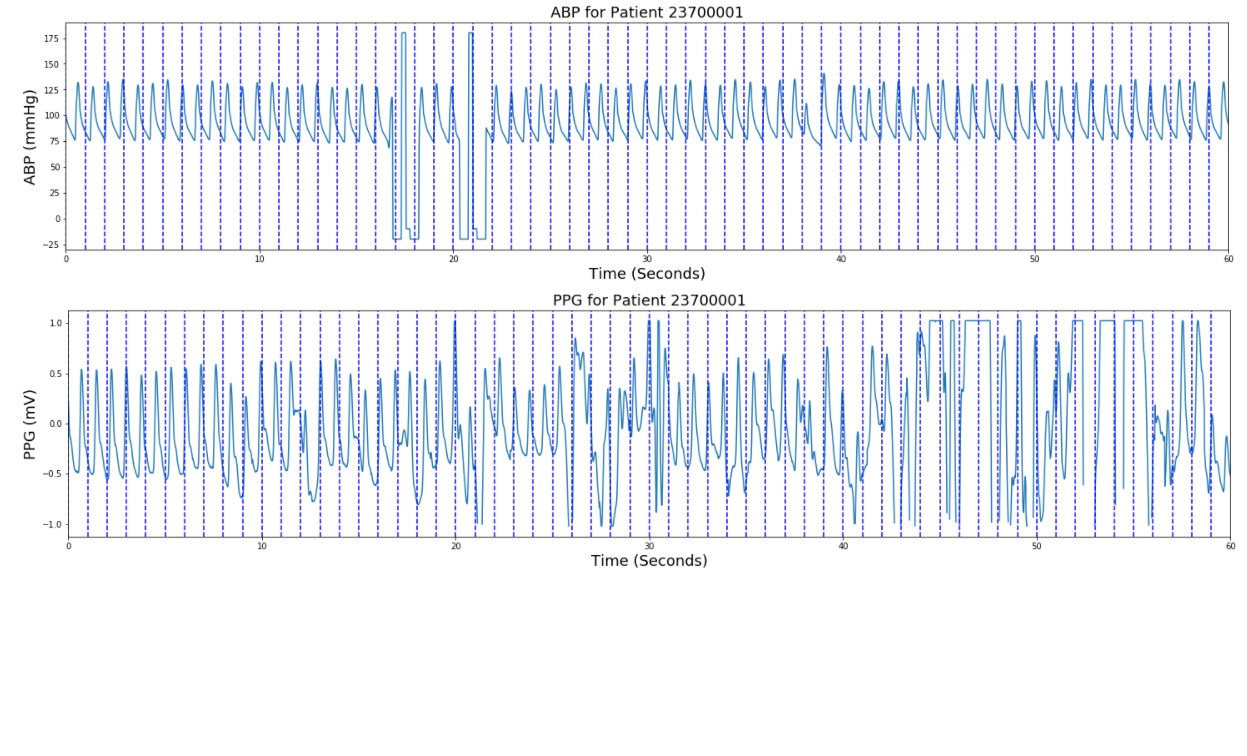
\includegraphics[width=16cm,height=16cm,keepaspectratio]{Implementation/window.png}
    \caption{Decision to window the signal}
    \label{windowing}
\end{figure}



\subsection{Stage 3: Choosing the patients}

\textcolor{red}{Why a subset? Why not all? If you're doing a split, explain this. Are you only using 8 patients out of the 90?}

Based on the decision to use a window length of 1 second, it was necessary to take a subset of the dataset. WHY? 
This was because a small window length means that a lot of datapoints are available for training already, so there 
is no need to acquire data from all 61 patients. By considering that the motivation of the FYP is to investigate the detection and prevention 
of hypertension, the decision was to examine the records of patients suffering with 
Cardiovascular diseases or other heart-related illnesses. Hence, a subset of the MIMIC I database was chosen, as illustrated 
in Table \ref{tabDatasetChosen}.
\begin{table}[H]
    \centering
    \caption{Characteristics of the chosen 12 patients from the MIMIC-I database}
    \label{tabDatasetChosen}
    \begin{tabular}{cccc}
    \hline
    \textbf{Patient record number} & \textbf{Age} & \textbf{Gender} & \textbf{Health condition} \\ \hline
    418 & 52 & M & CHF/pulmonary edema  \\
    480 & 52 & M & Post-op CABG         \\
    237 & 63 & F & MI/cardiogenic shock \\
    477 & 67 & M & Post-op CABG         \\
    466 & 70 & M & CHF/pulmonary edema  \\
    476 & 72 & F & Post-op CABG         \\
    225 & 73 & M & CHF/pulmonary edema  \\
    230 & 75 & F & CHF/pulmonary edema  \\
    213 & 82 & F & CHF/pulmonary edema  \\
    212 & 84 & M & CHF/pulmonary edema  \\
    456 & 84 & M & Post-op CABG         \\ 
    417 & 85 & M & CHF/pulmonary edema \\\hline
    \end{tabular}
\end{table}\noindent 



\begin{table}[H]
        \centering
        \caption{Number of samples available after initial preprocessing from the MIMIC database subset}
        \label{tabSamplesAvailable}
        \begin{tabular}{cc}
        \hline
        \textbf{Patient record number} & \textbf{10-minute Samples} \\ \hline
        418 &  0\\
        480 &  30\\
        237 &  17\\
        477 &  3\\
        466 &  139\\
        476 &  67\\
        225 &  17\\
        230 &  38\\
        213 &  42\\
        212 &  143\\
        456 &  83\\
        417 &  0\\ \hline
        \end{tabular}
\end{table}   

\subsection{Stage 4: Extracting the ground truth blood pressure values}
The ground truth Systolic and Diastolic blood pressure values are calculated by taking the respective 
maxima and minima of the arterial blood pressure signal within each window of the signal.

THEN TALK ABOUT PREPROCESSING APPLIED TO ABP




\subsection{Stage 5: Preprocessing the PPG signal}

\subsection{Stage 6: Processing of data before training}


\subsection{Stage 7: Overview of Neural Network models used}

\subsubsection{CNN AlexNet model}

\textcolor{red}{What type of information should the reader gather from this figure? It needs explaining and annotations/labelling.}

\begin{figure}[H]
    \centering
    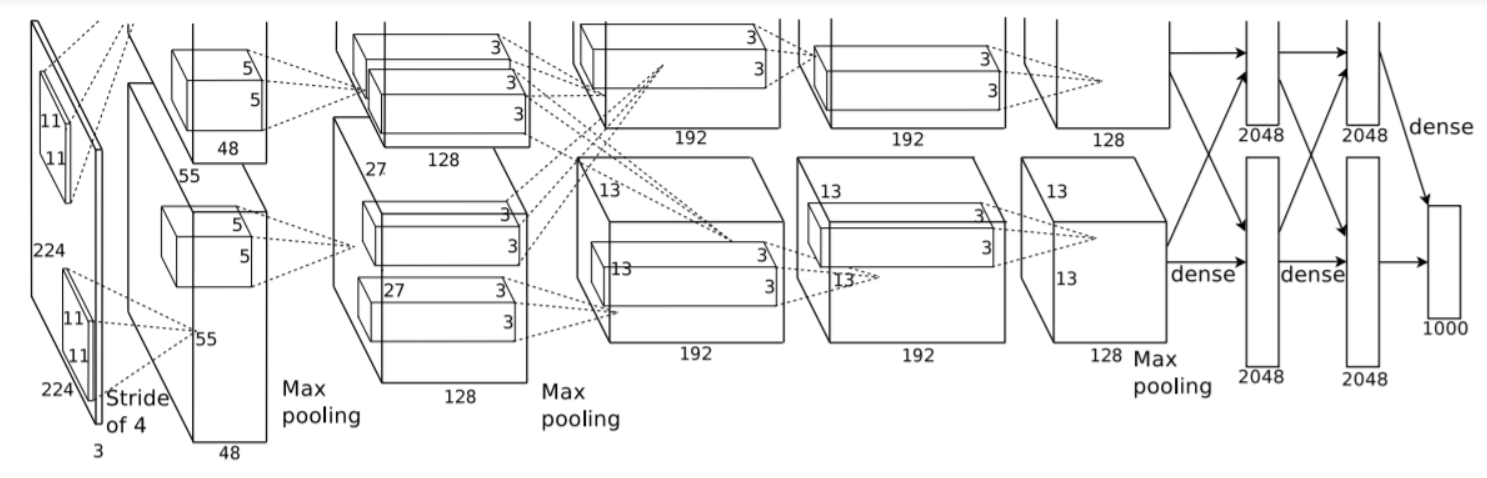
\includegraphics[width=10cm,height=10cm,keepaspectratio]{Implementation/alexnetArch.png}
    \caption{Overview of the AlexNet architecture}
    \label{alexnetArch}
\end{figure}

\subsubsection{CNN ResNet model}

\subsubsection{ResNet with LOSO model}

\subsubsection{LSTM model}

\subsubsection{Proposed Transformer Encoder model}


\subsection{Stage 8: Training the model}
PARAMETERS used

\subsection{Stage 9: How the error is evaluated}